% !TEX TS-program = pdflatex
% !TEX encoding = UTF-8 Unicode

% This is a simple template for a LaTeX document using the "article" class.
% See "book", "report", "letter" for other types of document.

\documentclass[11pt]{article} % use larger type; default would be 10pt
\usepackage{natbib}
\usepackage{mathtools}
\usepackage{graphicx}
\usepackage[colorlinks]{hyperref}
\usepackage[colorinlistoftodos, textwidth=4cm, shadow]{todonotes}



\usepackage[utf8]{inputenc} % set input encoding (not needed with XeLaTeX)


%%% Examples of Article customizations
% These packages are optional, depending whether you want the features they provide.
% See the LaTeX Companion or other references for full information.

%%% PAGE DIMENSIONS
\usepackage{geometry} % to change the page dimensions
\geometry{a4paper} % or letterpaper (US) or a5paper or....
% \geometry{margin=2in} % for example, change the margins to 2 inches all round
% \geometry{landscape} % set up the page for landscape
%   read geometry.pdf for detailed page layout information

\usepackage{graphicx} % support the \includegraphics command and options
\graphicspath{ {Graphics/} }
\usepackage{subfigure}

% \usepackage[parfill]{parskip} % Activate to begin paragraphs with an empty line rather than an indent

%%% PACKAGES
\usepackage{booktabs} % for much better looking tables
\usepackage{array} % for better arrays (eg matrices) in maths
\usepackage{paralist} % very flexible & customisable lists (eg. enumerate/itemize, etc.)
\usepackage{verbatim} % adds environment for commenting out blocks of text & for better verbatim
%\usepackage{subfig} % make it possible to include more than one captioned figure/table in a single float
% These packages are all incorporated in the memoir class to one degree or another...

%%% HEADERS & FOOTERS
\usepackage{fancyhdr} % This should be set AFTER setting up the page geometry
\pagestyle{fancy} % options: empty , plain , fancy
\renewcommand{\headrulewidth}{0pt} % customise the layout...
\lhead{}\chead{}\rhead{}
\lfoot{}\cfoot{\thepage}\rfoot{}

%%% SECTION TITLE APPEARANCE
\usepackage{sectsty}
\allsectionsfont{\sffamily\mdseries\upshape} % (See the fntguide.pdf for font help)
% (This matches ConTeXt defaults)

%%% ToC (table of contents) APPEARANCE
\usepackage[nottoc,notlof,notlot]{tocbibind} % Put the bibliography in the ToC
\usepackage[titles,subfigure]{tocloft} % Alter the style of the Table of Contents
\renewcommand{\cftsecfont}{\rmfamily\mdseries\upshape}
\renewcommand{\cftsecpagefont}{\rmfamily\mdseries\upshape} % No bold!

%%% END Article customizations


\title{Report \\ Automatic Polyphonic Piano Music Transcription}
\author{Agnieszka Szefer}
%\date{} % Activate to display a given date or no date (if empty),
         % otherwise the current date is printed 

\begin{document}

\newcommand{\myparagraph}[1]{\paragraph{#1}\mbox{}\\}
\maketitle

\listoftodos

\tableofcontents

\newpage


%%%%%%%%%%%%%%%%%%%
%%%%% INTRODUCTION %%%%%

\section{Introduction}
This chapter outlines the motivation behind the project, its main objectives and contributions. At the end of the section we describe a general outline of the report. 

\subsection{Motivation}
Even after millions of years of evolution of our sense of hearing it is still very difficult for a human without any prior musical education to tackle the problem of transcribing music, i.e. writing down the notes that make up a given piece of music. Furthermore, transcribing complex music pieces is a time-consuming task. Even for naturally talented people it may take several attempts to transcribe a whole piece correctly.

Automating the process of music transcription could be therefore of great help to musicians, especially to those lacking the skill of transcribing a piece `by ear'. There are large amounts of music that are not available in an annotated form. This includes traditional music passed from generation to generation or just released popular songs. Furthermore, there is an increasing community of people interested in learning how to play a piece from sheet music.
One of the most interesting applications of automated transcription is real time or offline feedback for music students. A student could see if what he or she plays is correct in respect to the sheet music he or she was given. \todo[inline]{Reference to Music Prodigy}%
\todo[inline]{Why piano music}%

\subsection{Objectives}
The aim of this project was to create an end-to-end system for automated transcription of piano music. In particular, we focused on correct detection of polyphonic music, it.e. where more than one note can be played at a time. We also investigated current state of the art methods for pitch detection and looked for ways to improve them in our system.
\todo[inline]{Improve the last sentence.}%

\subsection{Contributions}
In this report we complement the state of the art in automatic music transcription with the following contributions:

\begin{itemize}
\item We present an end-to-end solution to automatic music transcription. \todo[inline]{Can this be a contribution?}%
\todo[inline]{with user inferface maybe?} %
\item We introduce two techniques for finding noise threshold (one using least squares approach and another the total spectrum of significant spectral peaks) that improve the detection of pitch candidates.
\item We filter out insignificant spectral peaks in an early stage of transcription what improves the speed of pitch detection. \todo[inline]{Does it count as a separate contribution?}%
\item We show that using one FFT instead of commonly used STFT for each sound frame is `good enough' for pitch detection in our system and also requires less computations.
\item We experiment and test using real life data recorded by the author, where most of research papers test on studio recorded data.
\item We use user input data for better noise estimation and more accurate pitch detection. \todo[inline]{Is this a separate contribution?}%
\item We present challenges encountered in the development of the system and explain how we overcame them.
\item We evaluate our system and show its limitations, and suggest ideas for future work that could improve current transcription solutions.
\end{itemize}

\subsection{Report Outline}
\todo[inline]{Describe report outline}%

\newpage
%%%%%%%%%%%%%%%%%%
%%%%%BACKGROUND%%%%%
\section{Background}
This chapter introduces some concepts necessary to understand this project. We provide background in the area of digital signal processing and piano music.
We also describe the state of the art in the field of automated music transcription. 

%% Sound %%
\subsection{Sound}
Musical instruments or any other sources generate vibrations that are propagated through air or other medium in a form of a waveform. These vibrations are commonly known as \textit{sounds} and we are able to hear them because of the changes in the air pressure in our ears. If the pressure varies according to a repeating pattern we say that the sound has a \textit{periodic waveform} \citep*{Roads1996}.

One such pattern repetition is called a \textit{cycle}, and the \textit{fundamental frequency} is the number of cycles that occur per second. The frequency is measured in units of Hertz, where 1Hz means one cycle per second. The \textit{period} of a waveform is the lenght of the cycle and as it increases the frequency decreases.

Humans are usually able to hear frequencies in the range between 20Hz and 20000Hz.

\subsubsection{Sound Wave Representations}
One way of representing a sound waveform is as a time-domain graph showing how the air pressure changes over time (see Figure ~\ref{fig:representations}). The \textit{amplitude} is the maximum displacement of the wave measured from its equilibrium position.

A waveform may consist of not only the fundamental frequency, but also many other frequencies. The frequency-domain representation, also called the \textit{spectrum}, shows the frequencies that contribute to the sound (see Figure~\ref{fig:representations}). Any frequency component is a \textit{partial}. A partial that is an integer multiple of the fundamental frequency is called a \textit{harmonic}. If we assume a fundamental frequency of 440Hz, its second harmonic is 880Hz, third harmonic is 1760Hz, etc. Any frequency higher than the fundamental frequency is an \textit{overtone} (see Figure~\ref{fig:partials_harmonics}).

\begin{figure}[h!]
\begin{center}
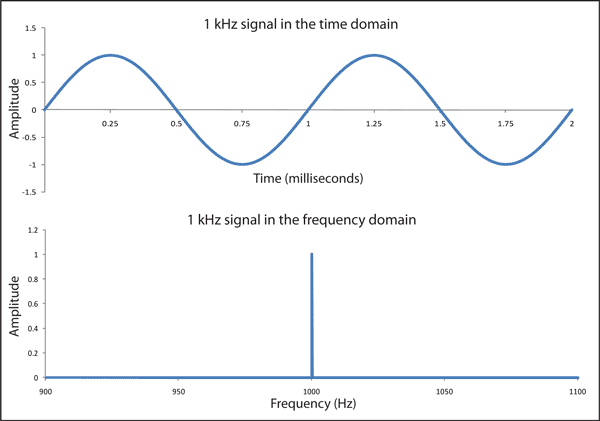
\includegraphics[scale=0.6]{TimeDomain}
\end{center}
\caption{Time-domain and frequency-domain representations of a sound wave.}
\label{fig:representations}
\end{figure}


\begin{figure}[h!]
\missingfigure{Fundamental frequency, partials, harmonics and overtones }
\caption{Fundamental frequency, partials, harmonics and overtones.}
\label{fig:partials_harmonics}
\end{figure}

%% Digital Signal %%
\subsection{Digital Signal}
Figure~\ref{fig:digital_recording} illustrates the process of digital audio recording and playback. A source generates sound waves. A microphone transduces the air pressure produced by this source into electrical voltages. The voltages are passed to analog-to-digital-converter (ADC). At each tick of the sample clock the ADC converts the voltages into strings of binary numbers.

\begin{figure}[h!]
\missingfigure{Overview of digital recording and playback see page 23 in Roads1996 }
%\caption{Overview of digital recording and playback.}
\label{fig:digital_recording}
\end{figure}

\subsubsection{Sampling}
In contrast to the analog signal (see Figure~\ref{fig:analog}), the digital signal is defined only at the points of time it has been \textit{sampled} at. In Figure~\ref{fig:digital} each vertical bar represents one sample of the signal. The \textit{sampling frequency} or \textit{sampling rate} is expressed in units of Hertz. In this project we experimented with signals sampled at the most common sampling frequency: 44.1 KHz with 16-bit samples. 
\todo[inline]{Mention aliasing and quantization error?}%
\todo[inline]{Some files were recorded at 48000Hz}%

\begin{figure}[h!]
\begin{center}
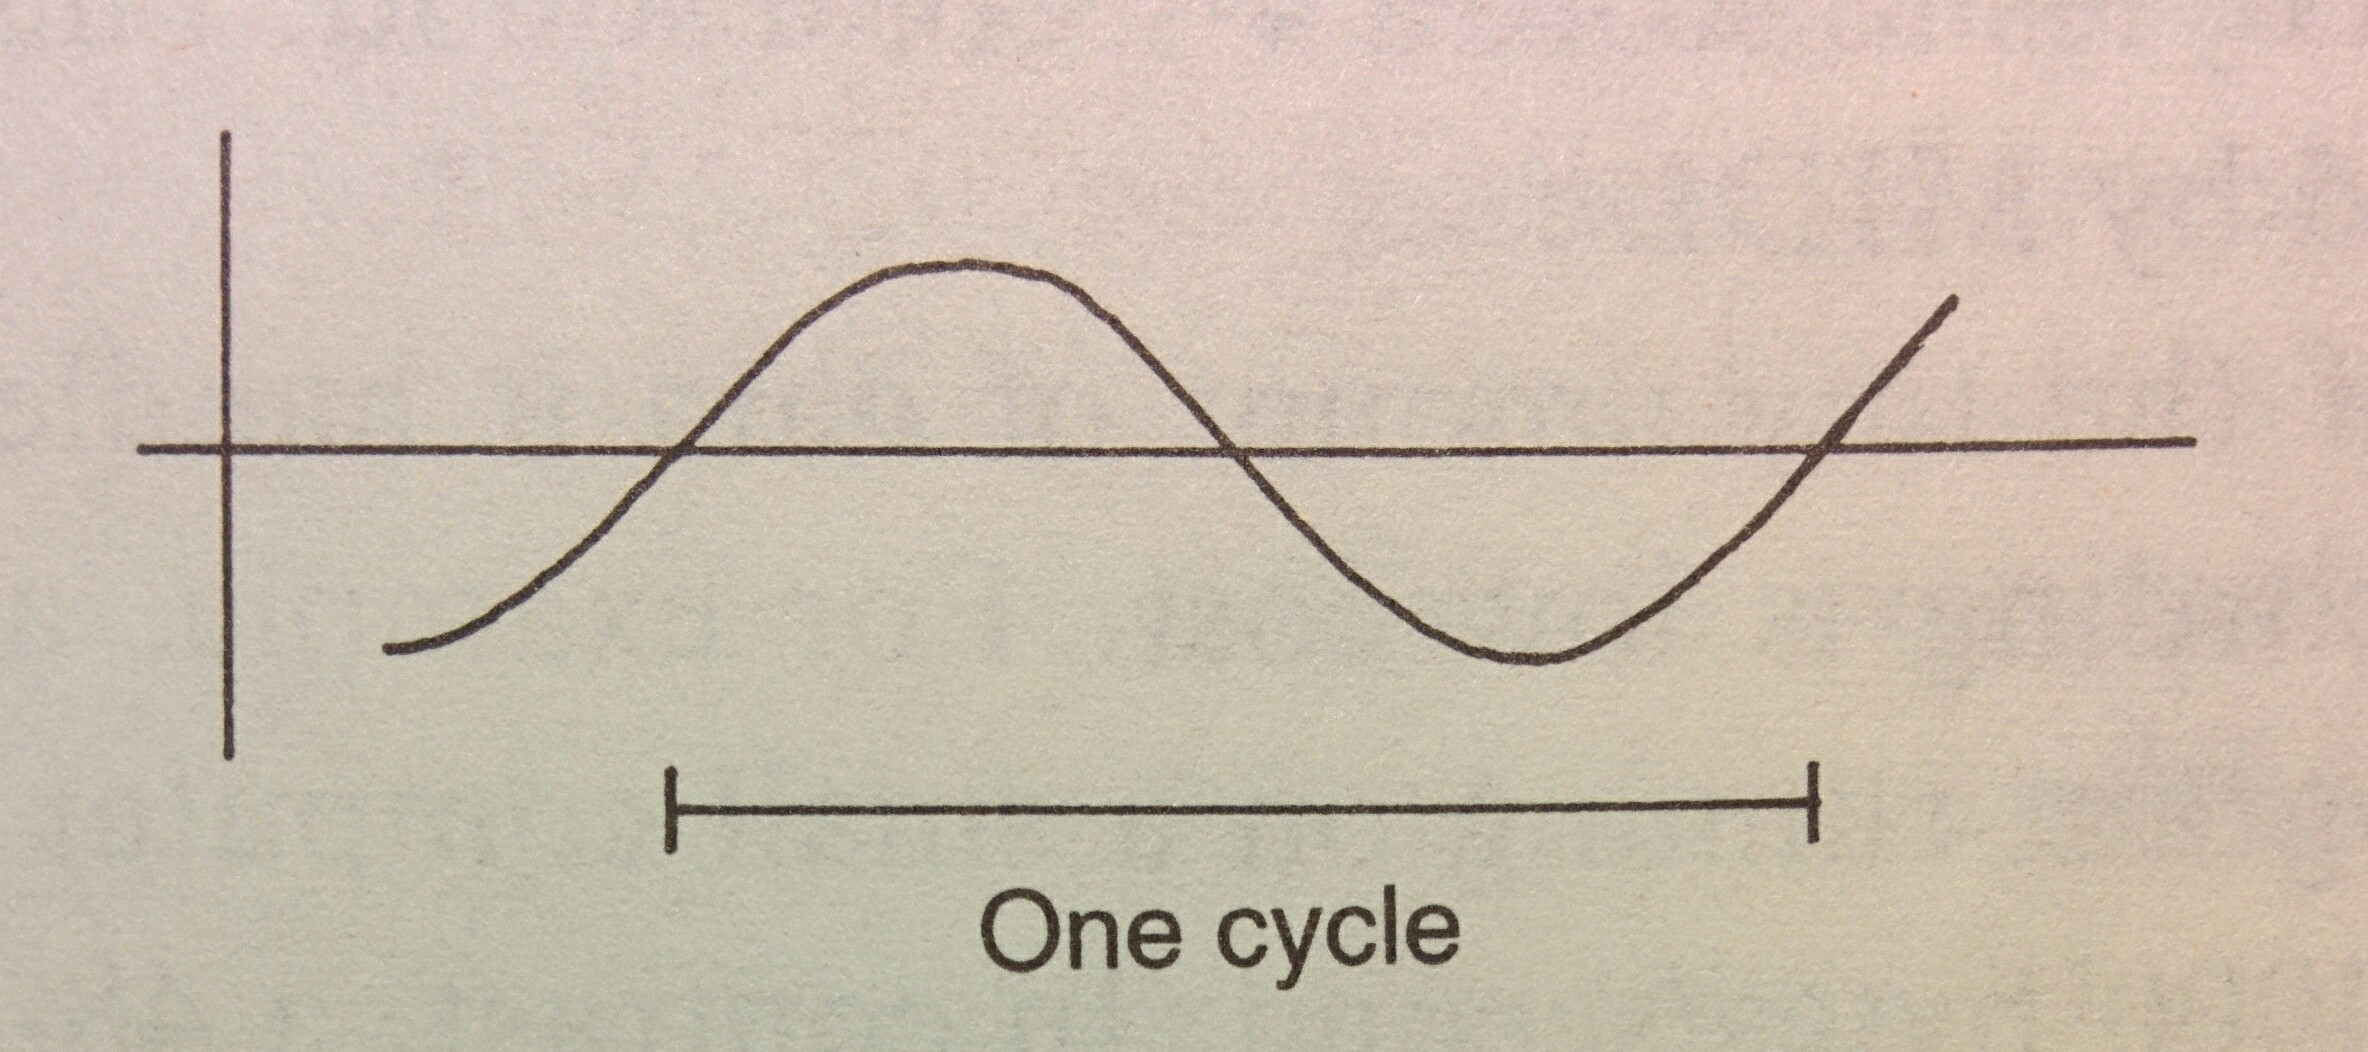
\includegraphics[scale=0.1]{analog}
\end{center}
\caption{Analog representation of a signal \citep*{Roads1996}.}
\label{fig:analog}
\end{figure}

\begin{figure}[h!]
\begin{center}
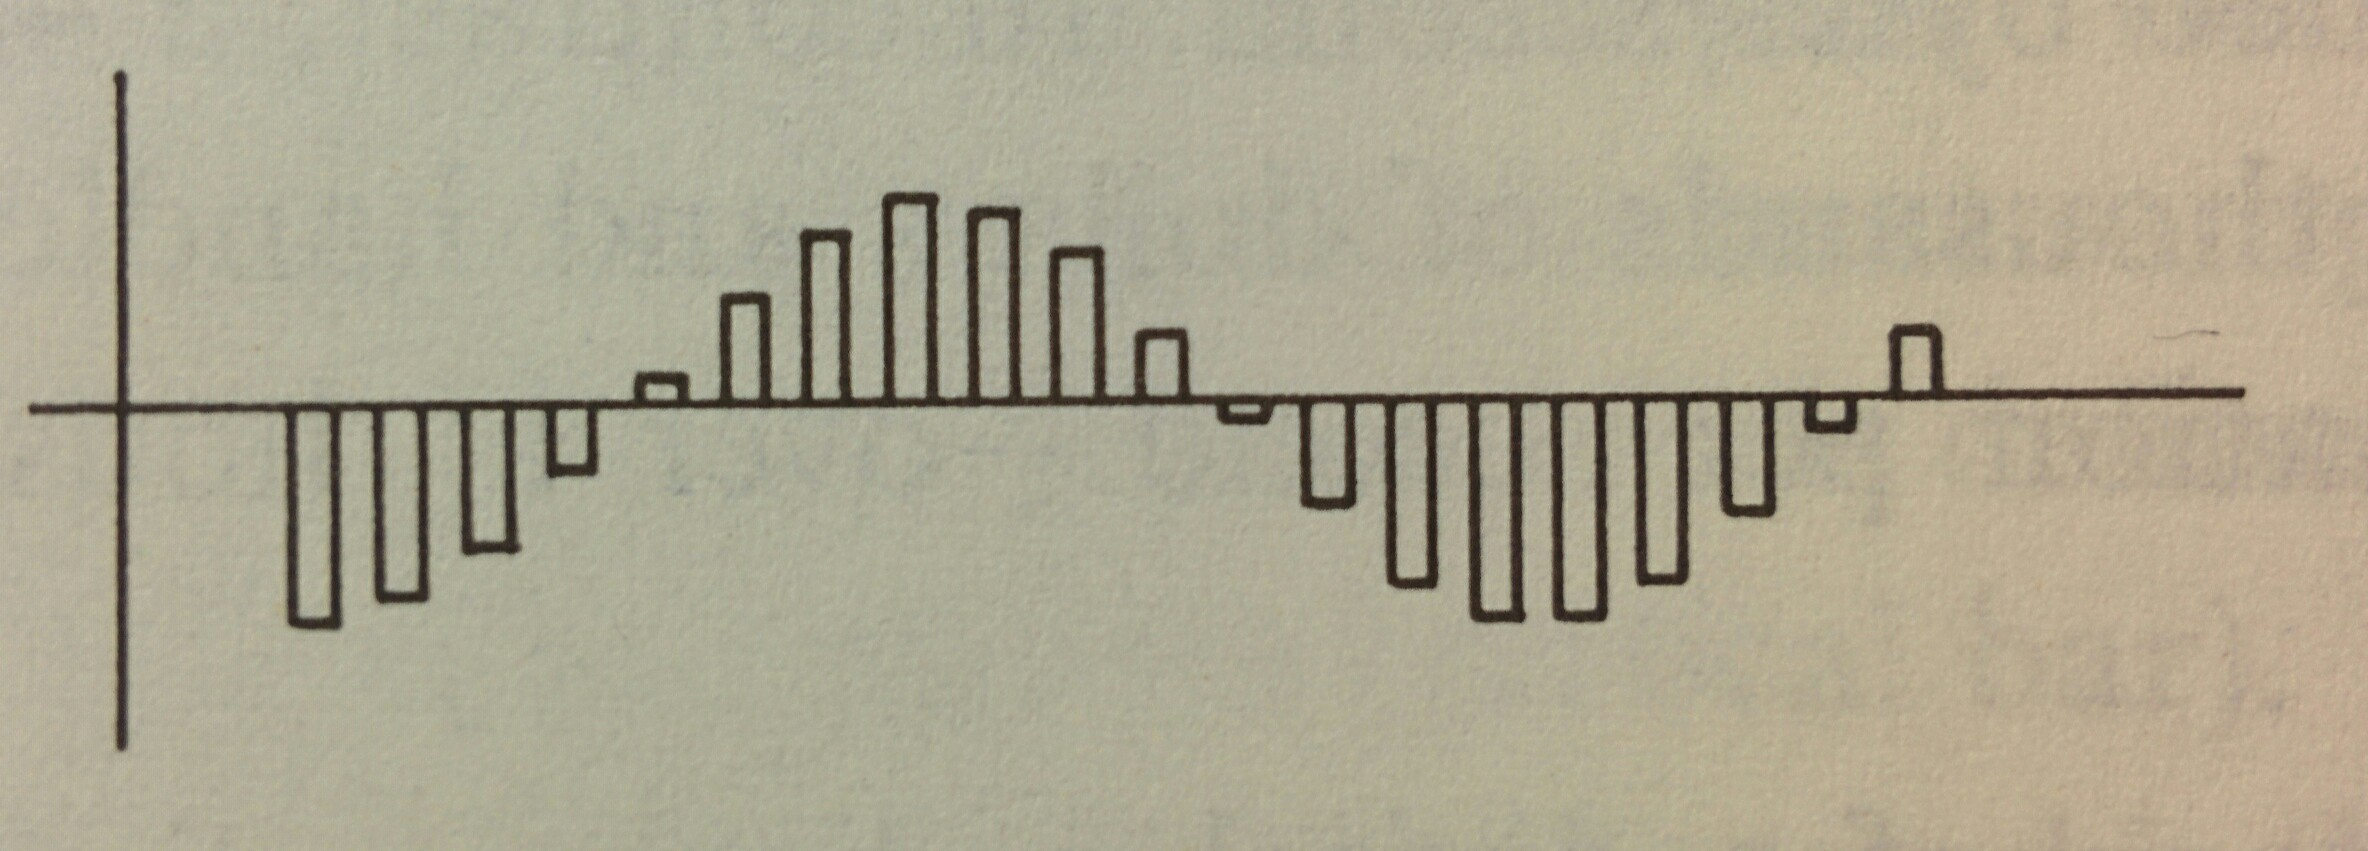
\includegraphics[scale=0.1]{digital}
\end{center}
\caption{Digital representation of a signal \citep*{Roads1996}.}
\label{fig:digital}
\end{figure}
\todo[inline]{Add labels to the diagrams.}

\subsubsection{WAVE Format}
\todo[inline]{It may be better to move it to Outline section and explain why this format is better than others.}
WAVE is an audio file format used for storing audio bitstreams. This format is uncompressed what ensures the highest quality of the recorded sound. Moreover, it is the most general music storage format and can be easily converted to other popular ones such as .mp3. 
\todo[inline]{Mention stereo (2 channels) vs. mono sound.}

%% MIDI %%
\subsection{MIDI}
MIDI is a popular protocol for control of digital music systems that allows for communication between an electronic instrument and a computer. In contrast to a digital audio recorder, a MIDI sequencer does not transmit the sampled waveform of the sound. When a music piece is played on a keyboard, a MIDI sequencer records only the start and ending time of each note, its pitch, and the amplitude of the beginning of a note. Therefore, AaStandard MIDI File (SMF) requires much less storage than .WAV to represent similar data.

For instance, if you play 4 quarter notes at a tempo of 60 beats per minute on a MIDI synthesizer, just 16 pieces of information of this 4-second sound are captured (4 starts, ends, pitches and amplitudes). On the other hand, if you record the same sound with a digital audio recorder set to a sampling frequency of 44.1 KHz, 352,800 pieces of information are recorded (44,100 * 2 channels * 4 seconds). Using 16-bit samples, it takes over 700,000 bytes to store a 4-second sound. This is 44,100 times more data than is stored by MIDI \citep*{Roads1996}. 

%% Piano %%
\subsection{Piano}
Piano is one of the most popular musical instruments. There are two types of pianos: a grand piano (Figure~\ref{fig:grand_piano}) and an upright piano (Figure~\ref{fig:upright_piano}). A piano has usually 88 keys (52 white and 36 black). The lowest note is A0 with a fundamental frequency of 27.5Hz and the highest one is C8 with a fundamental frequency at 4186.0 Hz. 

When you strike a piano key a padded hammer hits steel strings. The hammer rebounds and the strings continue to vibrate at their resonant frequency. When you release the key, a damper stops the string's vibration. 

\begin{figure}[h!]
\centering
\subfigure[A grand piano]{ 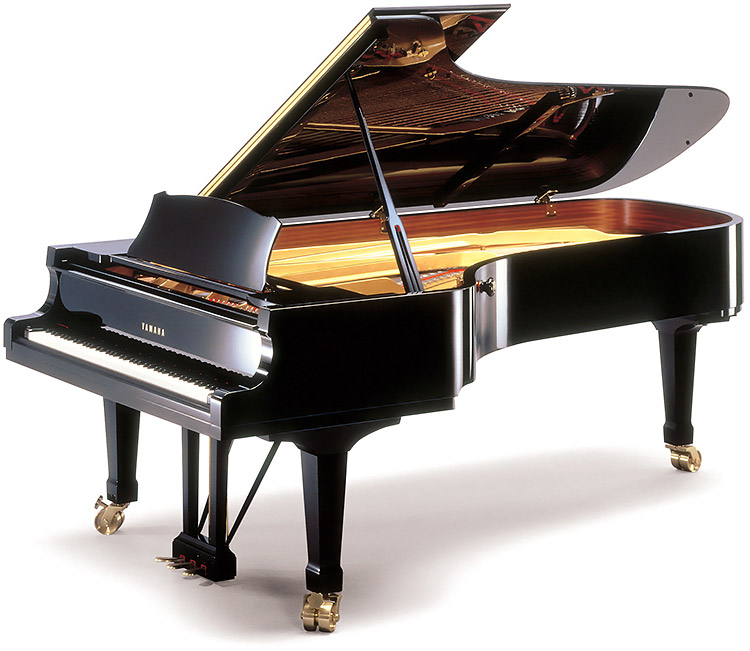
\includegraphics[scale=0.2]{grand_piano}\label{fig:grand_piano}}
\subfigure[An upright piano]{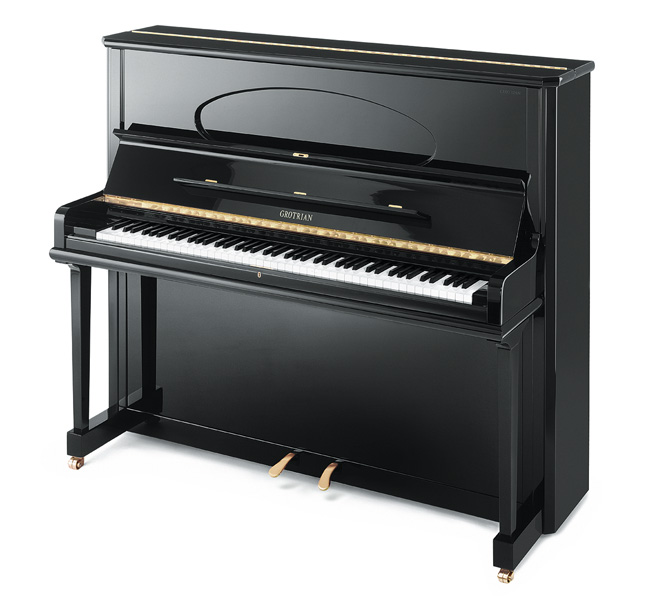
\includegraphics[scale=0.2]{upright_piano}\label{fig:upright_piano}}
\caption{Types of pianos.}
\label{fig:pianos}
\end{figure}

How the sound is made.

Inharmonicity.

Tuning.

Pedals.

\section{Outline}

\section{Details}

\section{Experiments}

\section{Evaluation}

\section{Conclusion}

\section{Further work}



\bibliographystyle{plainnat}
\newpage
\bibliography{references}

\end{document}


